\chapter{Grundlagen}
\section{Unternehmenseinführung in Capgemini} %VOrstellung von Capgemini(Geschichte, Zahlen, Wie groß?)
Capgemini, mit Hauptsitz in Paris, ist ein transnationales, börsennotiertes Unternehmen, das Beratungs-, Technologiedienstleistungen und digitale Transformationslösungen anbietet. Das Unternehmen bietet ein breites Spektrum an Services, darunter Beratung und Technologie. Mit einer Präsenz in über 50 Ländern bedient Capgemini Kunden aus diversen Branchen, einschließlich Finanzdienstleistungen, Automobilindustrie, Gesundheitswesen und Einzelhandel etc. Im Jahr 2024(Abb. \ref{Stand von Capgemini}) erzielte Capgemini einen Umsatz von 22,5 Milliarden Euro und beschäftigt weltweit etwa 340.000 Mitarbeiter.
\begin{figure}[h!]
	\begin{center}
		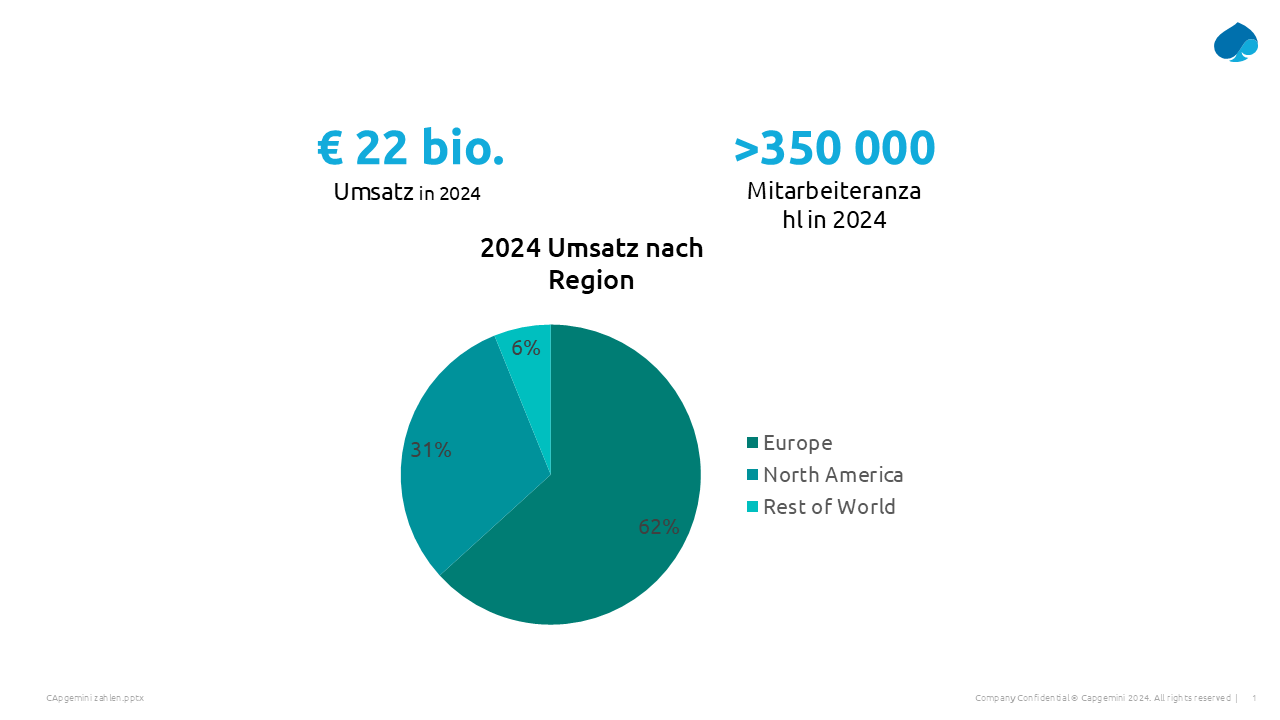
\includegraphics[width=8cm]{CApgemini zahlen.png}
		\caption{Volljähriges Finazbericht von Capgemini in 2024\cite{Capgemini_allgemein}}
		\label{Stand von Capgemini}
	\end{center}
\end{figure}
\subsection{Struktur und Organisation in Deutschland}

Capgemini Gruppe ermöglicht ihren Kunden eine umfassende IT-Transformation, die sämtliche Aspekte abdeckt – von der vollständigen Neugestaltung komplexer IT-Architekturen bis hin zur Entwicklung maßgeschneiderter, kleiner Funktionalitäten.  In diesem Zusammenhang verfügt Capgemini über große Mitarbeiteranzahl und besteht aus mehreren Marken:
\begin{itemize}
	\item \textbf{Capgemini Invent:} Diese Sparte konzentriert sich auf die strategische digitale Entwicklung der Kunden.\cite{Capgemini_invent}
	\item \textbf{Capgemini\cite{Capgemini}:} Das Mutterunternehmen bietet ein breites Spektrum an Dienstleistungen, darunter IT-Beratung.
	\item \textbf{Capgemini Engineering:} Ein weltweit führender Anbieter von Engineering- und F\&E-Dienstleistungen, der Kunden dabei unterstützt, ihren Weg zur Intelligent Industry zu beschleunigen.\cite{Capgemini_eng}
	\item \textbf{Sogeti:} Entwickelt, testet und schützt innovative Anwendungen für Unternehmen und stützt sich dabei auf Expertise in den Bereichen Beratung, Testen, agile und Cloud-Entwicklung sowie Cybersicherheit.\cite{Sogeti}
\end{itemize}
Dies sind die wichtigsten Marken von Capgemini in Deutschland. Wissenschaftliche Arbeit wurde im Mutterunternehmen von Capgemini durchgeführt, das intern in verschiedene Abteilungen gegliedert ist. Die Tätigkeit erfolgte in der Abteilung, die paketbasierte Lösungen für Kunden bereitstellt.

 %Im glossar erklären was PBS ist(SAP, Windchill etc.)
\section{Definition des End-2-End-Prozesses}
Ein End-to-End-Prozess (End-2-End) bezeichnet den Ablauf einer Aktion vom Anfang bis zum logischen Ende. Es gibt verschiedene End-to-End-Prozesse, die in Unternehmen betrachtet werden können. Zum Beispiel ist im Bereich Human Resources der sogenannte Hire-to-Retire-Prozess relevant, in der Logistik der Supply-Chain-Prozess und im Bereich des Product Lifecycle Management (PLM) der End-to-End-Prozess des Produktlebenszyklus.\cite{timinger2024modernes}%was anders????
\subsection{Überblick des allgemeinen End-2-End-Prozesses} %wie sieht algemein E2E-Prozess bei der Beratung!
%Wie bei allen Unternehmen ist die Hauptaufgabe der Consultingsunternehmen, den eigenen Unsatz und das Gewinn jährlich zu steigern. 
In dieser Arbeit wird der gesamte Prozess des Projektmanagements betrachtet. Das Projektmanagement besteht üblicherweise aus fünf Phasen(Abb. \ref{Projektmanagment}).\cite{timinger2024modernes}
\begin{figure}[h!]
	\begin{center}
		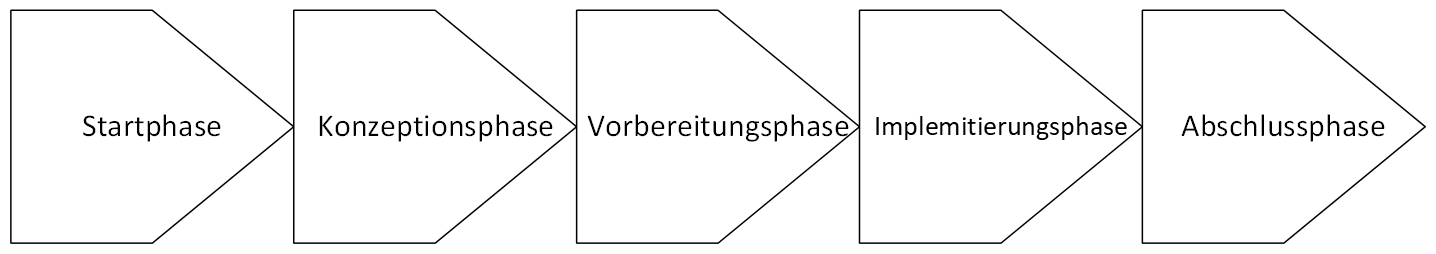
\includegraphics[width=12cm]{Drawing.png}
		\caption{Phasenplan eines Projektes\cite{timinger2024modernes}}
		\label{Projektmanagment}
	\end{center}
	
\end{figure}
\begin{enumerate}
	\item \textbf{Startphase:} 
	In dieser Phase erfolgt die Initiierung des Projekts, wobei die grundlegenden Ziele, Anforderungen und Nachfrage definiert werden. Die strategische Ausrichtung des Projekts wird durch die Fachbereichsleiter sowie die Stakeholder festgelegt.
	\item \textbf{Konzeptionsphase:}
	Auf Grundlage der definierten Ziele entwickeln die Projektleiter (z. B. die Leiter der Abteilungen IT, Ressourcenmanagement und HR) detaillierte Pläne und Konzepte zur Umsetzung des Projekts. In diesem Rahmen wird bestimmt, welche Mitarbeiter und Materialien erforderlich sind. Zudem wird überprüft, ob das Unternehmen über die benötigten Fachkräfte verfügt oder ob eine externe Rekrutierung notwendig ist.
	\item \textbf{Vorbereitungsphase:} 
	In dieser Phase werden die für die Projektdurchführung erforderlichen Ressourcen und Materialien beschafft sowie die organisatorischen Strukturen eingerichtet. Dabei übernehmen insbesondere der Projektleiter, das Beschaffungsteam und die Fachbereichsleiter eine zentrale Rolle, indem sie sicherstellen, dass alle notwendigen Ressourcen bereitgestellt werden.
	\item \textbf{Implementierungsphase:}  
	Die Umsetzung des Projekts erfolgt gemäß den zuvor entwickelten Plänen und Konzepten. Während dieser Phase überwachen der Projektleiter, das Projektteam und die Qualitätssicherung den Fortschritt, um die termingerechte und qualitativ hochwertige Durchführung des Projektes sicherzustellen.
	\item \textbf{Abschlussphase:} 
	Nach der Umsetzung wird das Projekt formal abgeschlossen. Dabei erfolgt eine Bewertung der Ergebnisse, und die Projektdokumentation wird erstellt. Zudem wird ein Plan zur Vermarktung des Produkts entwickelt, um eine effiziente Markteinführung und einen erfolgreichen Vertrieb sicherzustellen. Der Projektleiter, das Projektteam sowie die Stakeholder sind maßgeblich an der Evaluierung der Projektergebnisse, der Erstellung der Dokumentation und der Entwicklung der Verkaufsstrategie beteiligt.
	%REFERENZIEREN
\end{enumerate}
Jedes Projekt unterscheidet sich in Zielen, Inhalten und Dauer. Dennoch ist der Projektablauf meist ähnlich strukturiert. Typischerweise umfasst er die folgenden Phasen: Startphase, Konzeptionsphase, Vorbereitungsphase, Implementierungsphase, Abschluessphase. Diese allgemeinen Phasen ermöglichen eine systematische und effiziente Projektabwicklung, unabhängig von den spezifischen Unterschieden zwischen den Projekten\cite{wegmann2006projektmanagement}.
\subsection{End-2-End-Prozess bei Capgemini}
Capgemini ist ein Beratungsunternehmen, das keine eigenen Produkte entwickelt, sondern andere Unternehmen unterstützt. Aus diesem Grund unterscheidet sich das Projektmanagement und die Projektphasen von denen in Industrieunternehmen. In Abbildung \ref{Projektmanagment_Campgeini} sind die folgenden sechs Projektphasen definiert \cite{wegmann2006projektmanagement}:
\begin{figure}[h!]
	\begin{center}
		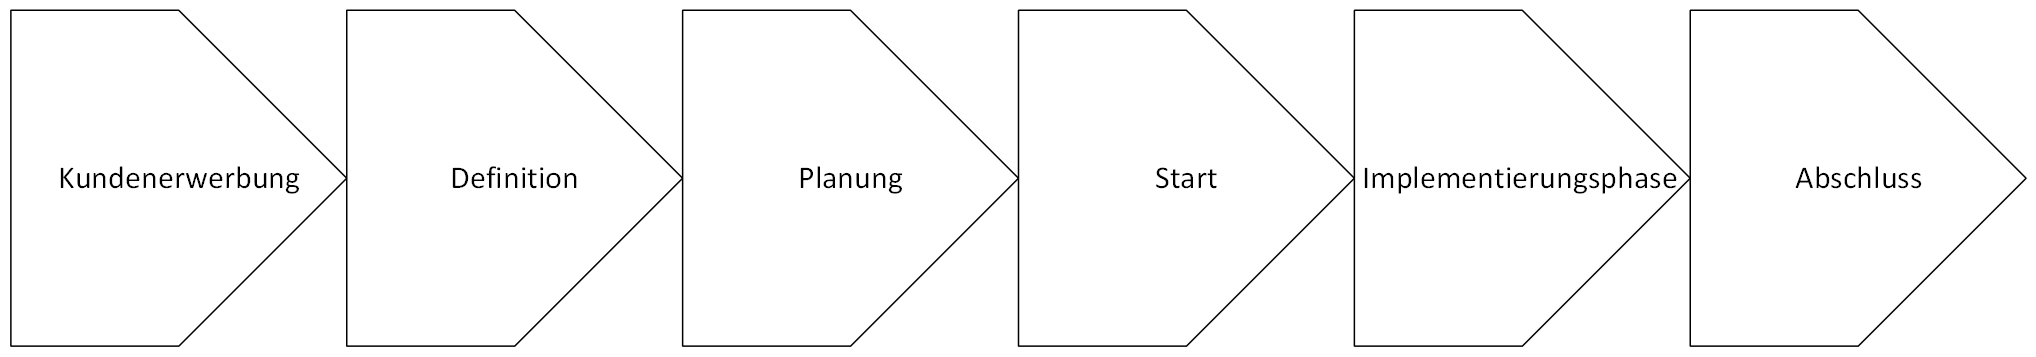
\includegraphics[width=12cm]{Projektmanagement_Capgemini .png}
		\caption{Phasenplan bei der Beratungsunternehmen(\textit{Kommentar an Jennifer: über alle Beratungsunternehmen} ) \cite{wegmann2006projektmanagement}}
		\label{Projektmanagment_Campgeini}
	\end{center}
\end{figure}
\begin{enumerate}
	\item \textbf{Kundengewinnung:} In dieser Phase bemüht sich die Vertriebsabteilung von 		Capgemini, neue Projekte zu akquirieren. Dabei werden verschiedene Strategien eingesetzt, wie die Demonstration der Fähigkeiten von Capgemini in relevanten Bereichen, die Hervorhebung erfolgreicher Referenzprojekte und die Präsentation von Innovationen auf Messen. Zusätzlich werden potenzielle Kunden durch gezielte Marketingmaßnahmen und persönliche Kontakte angesprochen, um die Beliebtheit von Capgemini zu stärken.
	\item \textbf{Definition des Projektes:} In dieser Phase recherchiert Capgemini, den Bedarf des Unternehmens zu definieren. Außerdem wird der Vertrag diskutiert und ausgearbeitet, um die Rahmenbedingungen und Erwartungen klar festzulegen.
	
	\item \textbf{Planung:} In dieser Phase wird das Projekt detailliert geplant. Es wird 
	festgelegt, wie viel Zeit für die Durchführung des Projekts benötigt wird und welche Rollen und Ressourcen erforderlich sind. Das Staffing-Team wählt entsprechend qualifizierte Mitarbeiter aus, um die Projektanforderungen zu erfüllen.
	\item \textbf{Start:} In dieser Phase versucht das ausgewählte Team, das Problem zu definieren und eine ausführliche Lösung zu erarbeiten. Dies umfasst die Erstellung eines detaillierten Zeitplans sowie die Festlegung der Verantwortlichkeiten für die einzelnen Aufgaben.
	\item \textbf{Implementierungsphase:} Dies ist die zeitlich umfangreichste Phase, in der alle Pläne in die Realität umgesetzt werden. Jeder Mitarbeiter führt seine spezifischen Aufgaben aus, um die Projektziele zu erreichen.
	\item \textbf{Abschluss:} In der Abschlussphase eines Projekts werden sämtliche organisatorischen und finanziellen Angelegenheiten zwischen dem Unternehmen und Capgemini geregelt. Gleichzeitig wird das Projekt offiziell an den Kunden übergeben, wodurch die Verantwortung vollständig auf diesen übergeht.
\end{enumerate}
\section{PLM-Systeme}
Zu Beginn des 21. Jahrhunderts wurde in der Fertigungsindustrie das Konzept des Product Lifecycle Managements (PLM) eingeführt. PLM dient der Überwachung und Steuerung von Produkten über deren gesamten Lebenszyklus hinweg und umfasst wesentliche Aktivitäten von Fertigungsunternehmen\cite{stark2011product}.
\subsection{Allgemeine Übersicht der PLM-Systeme}
Product Lifecycle Management (PLM) bezeichnet die Verwaltung des gesamten Lebenszyklus eines Produkts – von der Idee und Entwicklung über die Produktion und Nutzung bis hin zur Entsorgung oder zum Recycling. PLM kann sowohl ein einzelnes Produkt als auch das gesamte Produktportfolio eines Unternehmens verwalten\cite{stark2011product}.
\newline
Der Produktlebenszyklus kann aus mehreren Phasen bestehen, die jedoch in fünf Hauptphasen(Abb. \ref{PLM}) zusammengefasst werden können.
\begin{figure}[h!]
	\begin{center}
		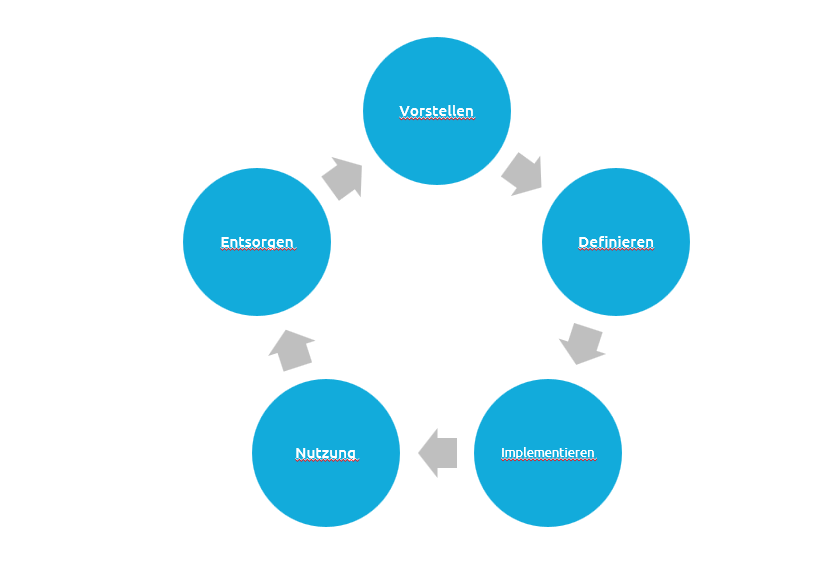
\includegraphics[width=12cm]{PLM.png}
		\caption{ Product Lifecycle Management\cite{stark2011product}}
		\label{PLM}
	\end{center}
\end{figure}
\begin{itemize}
	\item \textbf{Entwerfen:} In dieser Phase wird das Produkt entworfen. Das Unternehmen analysiert die Marktbedingungen sowie die voraussichtlichen Kosten für die Entwicklung des Produkts.
	\item \textbf{Definieren:} Hier wird die Entstehung des Produkts ausführlich geplant. Es wird ein Design skizziert, die Materialien für die Produktion werden festgelegt und andere technische Spezifikationen werden definiert.
	\item \textbf{Implementieren:} In dieser Phase beginnt die eigentliche Produktion des Produkts. Prozesse wie Montage, Qualitätskontrolle und Lieferkettenmanagement werden eingeführt.
	\item \textbf{Nutzen:} Das Produkt wird auf dem Markt verkauft und von den Kunden genutzt. Während dieser Phase stehen Kundenzufriedenheit, Wartung, Updates und Weiterentwicklungen im Fokus. Unternehmen sammeln Kundenfeedback, analysieren Leistungsdaten und bieten Support- oder Garantieprogramme an. Produktverbesserungen oder neue Versionen können aus dieser Phase hervorgehen.
	\item \textbf{Entsorgen:} In dieser Phase wird das Produkt vom Markt genommen. Unternehmen entwickeln Strategien für Recycling bzw. umweltfreundliche Entsorgung.
\end{itemize}
In einem Unternehmen liegt die Verantwortung für ein Produkt in den verschiedenen Phasen seines Lebenszyklus bei unterschiedlichen Abteilungen. Während in der frühen Phase des Produktlebenszyklus das Marketing eine zentrale Rolle spielt, übernimmt in der Entwicklungsphase primär die Konstruktions- und Ingenieurabteilung die Verantwortung. In späteren Phasen, insbesondere während der Nutzung des Produkts, sind der Kundenservice und die Wartungsabteilung maßgeblich involviert. Die Produktion kann auch in verschiedenen Ländern stattfinden.
Daher treten Unternehmen bei der Entwicklung des Produkts auf mehrere Probleme, wie den Verlust der Kontrolle über die Produktion(z.B. fehlende Bestandteile), was zu einer sinkenden Qualität führen kann. Zudem gibt es möglicherweise keine Möglichkeiten, das Produkt an verschiedenen Standorten zu fertigen\cite{stark2011product}.\newline
Ein Product Lifecycle Management (PLM)-System kann diesen Herausforderungen entgegenwirken, indem es eine zentrale Plattform für die Verwaltung und den Austausch produktbezogener Daten bietet. Durch die Standardisierung von Prozessen und eine einheitliche Datenbasis ermöglicht PLM-System eine effizientere Zusammenarbeit zwischen den Fachabteilungen, verbessert die Nachverfolgbarkeit von Produktänderungen und unterstützt fundierte Entscheidungsprozesse über den gesamten Lebenszyklus hinweg\cite{ozturk2019product}.
\subsection{Vorstellung von verschiedenen Vendoren}
Auf dem Markt existieren viele verschiedene PLM-Systeme, auch sogenannte PLM-Vendoren. Dies sind Unternehmen, die spezialisierte Softwarelösungen entwickeln, die auf unterschiedliche Branchen, Unternehmensgrößen und Anforderungen zugeschnitten sind. Sie bieten PLM-Software an, um technische produktbezogene Inhalte zu erfassen, zu pflegen und zu verwalten. Diese Inhalte definieren die Produktspezifikationen und -designs sowie die zulässigen Produktkonfigurationen\cite{PLM1}.
Im Jahr 2023 wuchs der globale Markt für Product Lifecycle Management und Engineering (PLM)-Software auf nahezu 28,4 Milliarden US-Dollar, was einem Wachstum von 9,6\% im Vergleich zu 2022 entspricht. Die zehn größten Anbieter hielten einen bedeutenden Marktanteil von 85,7\%, wobei Dassault Systèmes mit 17,1\% führend war. Hier sind die Top-10 PLM-Vendoren im Jahr 2023 auf dem Markt\cite{Top10PLMVendoren}:
\begin{enumerate}
	\item \textbf{Dassault Systèmes} 
	\item \textbf{Autodesk}
	\item \textbf{Synopsys}
	\item \textbf{Siemens Digital Industries Software}
	\item \textbf{Cadence Design Systems}
	\item \textbf{PTC}
	\item \textbf{Hexagon}
	\item \textbf{ANSYS}
	\item \textbf{Altair}
	\item \textbf{Bentley Systems}
\end{enumerate}
Capgemini bietet die Implementierung von PLM-Systemen für ihre Kunden an und arbeitet dabei hauptsächlich mit vier Anbietern zusammen: Dassault Systèmes, PTC, Siemens Digital Industries Software und Aras. Wie schon erwäht, bieten diese Unternehmen zunächst zentrumbildende PDM-Softwarelösungen.
\begin{itemize}
	\item \textbf{Dessault Systemes:} Ein französisches Softwareunternehmen, das sich auf 3D-Design, Simulation und  PLM spezialisiert hat. Es wurde 1981 gegründet und ist bekannt für seine 3DEXPERIENCE-Plattform, die in verschiedenen Industrien wie Luft- und Raumfahrt, Automobil und Medizintechnik eingesetzt wird\cite{Dessault}.
	\item \textbf{PTC(Parametric Technology Corporation):} Ein US-amerikanisches Unternehmen mit Sitz in Boston, das 1985 gegründet wurde. PTC bietet Softwarelösungen für CAD (Creo), PLM (Windchill) und IoT (ThingWorx) an. Besonders stark ist PTC in der digitalen Transformation und der Integration von Augmented Reality (Vuforia) in industrielle Prozesse\cite{PTC}.
	\item \textbf{Siemens Digital Industries Software:} Ein Tochterunternehmen von Siemens mit Sitz in Plano, Texas, das sich auf 3D- und 2D-PLM-Software spezialisiert hat.  Eine der wichtigsten PLM-Lösungen von Siemens ist Teamcenter, das als zentrale Plattform für Produktdaten- und Prozessmanagement fungiert\cite{Siemens}.
	\item \textbf{Aras:} Ein amerikanischer Entwickler und Herausgeber von Produktentwicklungssoftware\cite{Aras}.
\end{itemize}
 